\section{Description du plastique}
\par{
Le plastique est un terme qui d\'esigne des mat\'eriaux divers issus de la transformation de produits organiques de synth\`ese tels que le p\'etrole, le charbon, le gaz naturel qui sont utilis\'es dans de nombreuses applications. Le plastique ou mati\`ere plastique est une substance synth\'etique polym\`ere contenant un grand nombre d'atomes de carbone, oxyg\`ene, hydrog\`ene ou azote. Il en existe deux cat\'egories: les thermoplastiques et les thermodurcissables. Les thermoplastiques se ramollissent sous la chaleur permettant leur moulage et durcissent lors du refroidissement. Les thermodurcissables, une fois moul\'es, conservent leur forme d\'efinitive {\citep{Valorplast}}. Bien que de nombreuses mati\`eres plastiques soient disponibles dans le commerce, seulement certaines d'entre elles se qualifient comme mati\`eres thermoplastiques. Les principales sont le poly\'ethyl\`ene basse densit\'e (PEBD), le poly\'ethyl\`ene haute densit\'e (PEHD), le polypropyl\`ene (PP), le chlorure de polyvinyle (PVC), le polystyr\`ene (PS) et le poly\'ethyl\`ene t\'er\'ephtalate (PET). Ils repr\'esentent environ 90\% de la demande totale {\citep{andrady2009applications}}
}

\subsection{Caract\'eristiques chimiques}
\par{
La mati\`ere de base du plastique est un polym\`ere. On peut classer les polym\`eres selon qu'ils sont naturels provenant du r\`egne animal ou v\'eg\'etal comme la cellulose ou le caoutchouc ou artificiels, obtenus par transformation chimique de polym\`eres naturels ou encore synth\'etiques obtenus par polym\'erisation de monom\`eres. Les polym\`eres sont un  syst\`eme form\'e par un ensemble de macromol\'ecules, entit\'es mol\'eculaires de grande taille issues de l'assemblage covalent d'un grand nombre d'unit\'es monom\`eres r\'ep\'etitives. Les macromol\'ecules ainsi form\'ees, plus grandes que les mol\'ecules simples, apporte au polym\`ere de nouvelles propri\'et\'es, comme la viscosit\'e ou la r\'esistance, que l'on pourra utiliser dans la fabrication de nombreux produits. Le nombre d'unit\'es monom\`eres qui constitue le polym\`ere est appel\'e le degr\'e de polym\'erisation. La masse molaire du polym\`ere est donc directement li\'ee au degr\'e de polym\'erisation. Les polym\`eres synth\'etiques sont donc issus de la polym\'erisation {\citep{fontanille2014chimie}}.
}

\begin{figure}[h]
\centering
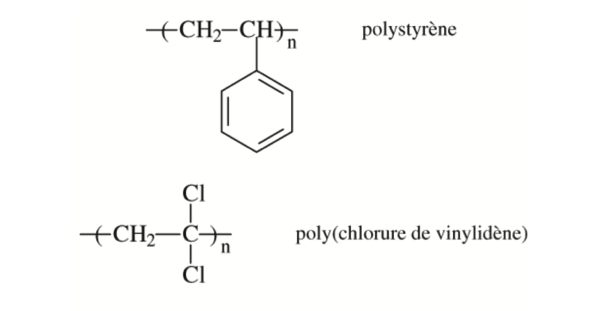
\includegraphics[scale=0.8]{Structurepoly.png}
\caption{Exemples de structure chimique de compos\'es polym\`eres. {\citep{fontanille2014chimie}}} 
\label{structurepoly}
\end{figure}
\FloatBarrier
\par{
Un polym\`ere form\'e d'unit\'es monom\`eres identiques est un homopolym\`ere tandis qu'on le nommera co-polym\`ere s'il pr\'esente des unit\'es monom\`eres de deux ou plusieurs sortes diff\'erentes. Les polym\`eres peuvent \^etre class\'es selon leur structure et peuvent pr\'esenter des architectures lin\'eaires, ramifi\'ees ou r\'eticul\'ees. Les polym\`eres peuvent \^etre monodimensionnels et donc lin\'eaires, r\'esultant de la polym\'erisation des monom\`eres bivalents.
}

\begin{figure}[h]
\centering
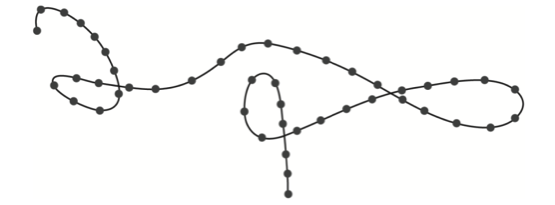
\includegraphics[scale=0.8]{Chainepoly.png}
\caption{Repr\'esentation de a cha\^ine d'un polym\`ere lin\'eaire. {\citep{fontanille2014chimie}}} 
\label{chainepoly}
\end{figure}
\FloatBarrier
\par{
Ils peuvent \'egalement \^etre bidimensionnels essentiellement produits par la nature ou tridimensionnels soit naturels soit r\'esultant de la polym\'erisation de monom\`eres dont la valence est sup\'erieure \`a deux ou encore par r\'eticulation de polym\`eres lin\'eaires par voie chimique ou physique. Leur dimension mol\'eculaire est infinie {\citep{fontanille2014chimie},\citep{Valorplast}}.
}
\begin{figure}[h]
\centering
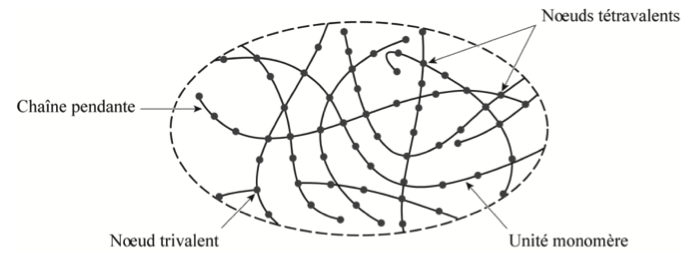
\includegraphics[scale=0.8]{poly3d.png}
\caption{Repr\'esentation sch\'ematique d'un polym\`ere tridimensionnel. {\citep{fontanille2014chimie}}} 
\label{poly3d}
\end{figure}
\FloatBarrier

\par{
La dimensionnalit\'e des polym\`eres influencent leurs propri\'et\'es comme c'est le cas des propri\'et\'es m\'ecaniques. La  plupart  des  propri\'et\'es  des  polym\`eres,  qui  sont  exploit\'ees  dans  une  tr\`es  grande  vari\'et\'e d'applications,  sont  \'etroitement  li\'ees  \`a  leur  coh\'esion.  Celle-ci  d\'epend  essentiellement  de l'intensit\'e des interactions mol\'eculaires qui se d\'eveloppent entre groupements mol\'eculaires. La polym\'erisation peut se faire par \'etapes de type polycondensation ou polyaddition comme c'est le cas pour des mol\'ecules lin\'eaires thermoplastiques ou des mol\'ecules r\'eticul\'ees thermodurcissables. La polym\'erisation en cha\^ine est un autre type de r\'eaction de polym\'erisation soit radiculaire, soit ionique comme c'est le cas du polystyr\`ene {\citep{fontanille2014chimie}}. Les plastiques sont rarement utilis\'es tels quels. Les r\'esines sont m\'elang\'ees avec d'autres mat\'eriaux appel\'es "additifs" pour modifier ou am\'eliorer leurs propri\'et\'es et donc leur performance. Ceux-ci peuvent comprendre des charges inorganiques (par exemple du carbone ou de la silice) pour renforcer la mati\`ere plastique, des stabilisants thermiques pour permettre le traitement des mati\`eres plastiques \`a des temp\'eratures \'elev\'ees, des plastifiants pour rendre le mat\'eriau flexible et souple, des ignifugeants pour \'eviter la combustion, ainsi que des protecteurs solaire pour \'eviter la d\'egradation lorsqu'ils sont expos\'es \`a la lumi\`ere du soleil. D'autres produits ou colorants peuvent \'egalement \^etre utilis\'es pour am\'eliorer l'aspect du plastique {\citep{andrady2009applications}}.
}

\subsection{Caract\'eristiques physiques}
\subsubsection{Propri\'et\'es thermiques}

\par{
Les polym\`eres sont dits thermostables lorsqu'une utilisation \`a long terme est possible \`a des temp\'eratures relativement \'elev\'ees, dans le cas o\'u la temp\'erature de transition vitreuse est \'elev\'ee, ou si le taux de cristallinit\'e \'elev\'e, en m\^eme temps qu'une temp\'erature de fusion \'elev\'ee, sont coupl\'es \`a une stabilit\'e chimique en temp\'erature. Cette appellation peut concerner \`a la fois les polym\`eres thermoplastiques et les polym\`eres thermodurcissables {\citep{domin2013}}. A l'\'etat fondu, le polym\`ere devient mall\'eable ce qui permet de les mouler. A la chaleur il peut se transformer de fa\c con r\'eversible en \'etat solide ou liquide.
}
\par{
Ainsi, les polym\`eres sont durs et rigides \`a temp\'erature ambiante: c'est l'\'etat vitreux et sont mous et flexibles \`a une certaine temp\'erature qui est propre aux diff\'erents polym\`eres g\'en\'eralement autour de 120\degree C. Ils ont des propri\'et\'es visco\'elastiques d\'ependant de la temp\'erature. Il existe une temp\'erature de transition vitreuse. Les polym\`eres thermodurcissables \'etant r\'eticul\'es, l'augmentation de la temp\'erature ne permet pas de rompre, de mani\`ere r\'eversible, les liaisons covalentes qui les relient car les liaisons des cha\^ines primaires se briseraient aussi. Il n'est donc pas possible de les ramollir en \'elevant la temp\'erature {\citep{lecomte2009physique}}.
}

\subsubsection{Propri\'et\'es m\'ecaniques}
\par{
La propri\'et\'e m\'ecanique principale est le fait que les polym\`eres sont "plastiques". Cette propri\'et\'e \'elastique des polym\`eres d\'epend de la nature de la cha\^ine ainsi que de sa longueur, de son niveau d'enchev\^etrement et fait entrer en ligne de compte les forces qui s'y appliquent et qui entrainent des d\'eformations. Une structure de cha\^ines r\'eguli\`ere va pouvoir s'empiler pour former un r\'eseau cristallin tridimensionnel plus facilement que dans le cas de cha\^ines de structure d\'esordonn\'ee. Lorsque les cha\^ines du polym\`ere sont dispos\'ees de fa\c con al\'eatoire, qu'elles sont tordues, le polym\`ere est dit amorphe et il est transparent. Les \'elastom\`eres sont des polym\`eres amorphes. Ils sont souples et d\'eformables  \`a temp\'erature ambiante. Un polym\`ere form\'e de fa\c con lin\'eaire est tr\`es cristallin ce qui leur donne rigidit\'e et translucidit\'e {\citep{lecomte2009physique}}.
}

\subsubsection{Autres propri\'et\'es}
\par{
La plupart des polym\`eres sont de bons isolants \'electriques (r\'esistivit\'e \'electrique $\approx 1020 \mu ohm.cm$). Au niveau optique, la transparence des polym\`eres d\'epend fortement de l'\'etat structural: les polym\`eres purs et non cristallins sont souvent transparents. Les polym\`eres semi-cristallins sont soit translucides soit opaques. Les polym\`eres peuvent pr\'esenter des propri\'et\'es toxicologiques. Elles peuvent \^etre dues \`a une cha\^ine de polym\`eres qui se d\'ecompose ou \`a la volatilit\'e due \`a des additifs  {\citep{lecomte2009physique}}.
}